\documentclass[10pt,english,a4paper]{article}
\newcommand{\dir}{.}
\newcommand{\commondir}{../common}
\usepackage{fancyhdr}
\usepackage{fancybox}
\usepackage{babel}
\usepackage{a4}
\usepackage[round]{natbib}
\usepackage{graphicx}
\usepackage{supertabular}
\usepackage{amsfonts}
\usepackage{amsthm}
\usepackage{eucal}
\usepackage[intlimits]{amsmath}
\usepackage{ifthen}
\usepackage{url}
\usepackage{alltt}

\usepackage{color}
\usepackage[colorlinks=true,citecolor=blue,dvipdfm]{hyperref}
%\date{6th October 2005}

\newboolean{html}
\setboolean{html}{false}

\newcommand{\pd}{\partial}
\renewcommand{\vec}{\boldsymbol}

\setlength{\oddsidemargin}{1.35cm} %margins set up for psglg1
\setlength{\evensidemargin}{-0.1cm}
\setlength{\topmargin}{0cm}
\setlength{\textwidth}{14.55cm}
\setlength{\textheight}{22.3cm}

% implement href as a footnote
\begingroup% 
\ifx\href\undefined%
\gdef\href#1#2{%
#2\footnote{\url{#1}}%
}%
\fi\endgroup%

% environment for PyCF cookbook
\newcommand{\pycffigure}{}
\newenvironment{pycf}[2] %
{\renewcommand{\pycffigure}{#2}
 \begin{center}
 \begin{tabular}{p{0.65\textwidth}c}
 \multicolumn{2}{p{\textwidth}}{\tt #1}\\
 \begin{minipage}[t]{0.65\textwidth}
 \vspace{0pt}
}%
{\end{minipage} &
 \begin{minipage}[t]{0.35\textwidth}
 \vspace{0pt}
 \includegraphics[width=0.9\textwidth]{\pycffigure}
 \end{minipage}\\
 \end{tabular}
 \end{center}
}

\bibliographystyle{plainnat}

\input{common/version.tex}




\pagestyle{myheadings}

\markright{Glimmer-CISM Branches}

\begin{document}
\title{Glimmer-CISM Branches}
\author{Magnus Hagdorn\thanks{Magnus.Hagdorn@ed.ac.uk}}

\maketitle

2010 will be an exciting year for Glimmer-CISM development. We plan to make a release of the model with the higher order physics included. There are also plans for a major refactoring effort to make the ice sheet model more modular.

\begin{figure}[htbp]
\centering
\includegraphics[width=\textwidth]{\dir/figs/gc-branches.eps}
\caption{Glimmer-CISM branches and merge points for 2010}
\end{figure}

The diagram above illustrates the relationship among various existing branches and branches to be created. We have the following plans:
\begin{enumerate}
\item {\bf April 2010} merge Bill's changes on the GC2-gcm branch into GC2-trunk and make a GC-1.6 release. This series of stable releases will be integrated into CCSM.
\item {\bf End of April 2010} merge GC-lanl-trunk into GC2-trunk and make a GC-1.8 release. This series of stable releases will contain the higher order physics but no parallelisation
\item {\bf Summer 2010} finish refactoring of shallow ice glimmer and merge GC2-refactoring into GC2-trunk. 
\item refactor higher order parts of Glimmer-CISM. Once ready make GC-2.0 release.
\item create new GC2-parallel branch and merge in differences between GC-lanl-parallel and GC-lanl-trunk. The parallel branches will remain private for now.
\end{enumerate}

\end{document}
